\noindent Recommended references:

\begin{itemize}
\item \textit{A Mathematical Introduction to Conformal Field Theory} by Schottenloher.
\item \textit{Applied Conformal Field Theory}, hep-th/9108028, by Ginsparg.
\item \textit{Conformal Field Theory} (``Yellow Book'') by Francesco, Mathieu, Senechal.
\end{itemize}

\noindent Why study conformal field theory (CFT)?

\begin{itemize}
\item CFT provides a good description of systems at or near criticality.
\item CFTs are the only true quantum field theories (QFTs), since they are cutoff-independent. One can think of QFTs as perturbations of CFTs. CFTs correspond to renormalization groups of fixed points, which dominate an effective theory at or near criticality.
\item CFTs can be made, by and large, mathematically rigorous, at least in $(1+1)$-dimensional theories. There are three major competing mathematical descriptions for CFT, and advances are being made towards a single, unifying description.
\end{itemize}

\noindent Prerequisites for this material:

\begin{itemize}
\item Advanced quantum mechanics
	\subitem E.g, many-body theory and Fock spaces.
\item Classical field theory
	\subitem E.g., symplectic geometry.
\item Quantum field theory.
\item Advanced quantum field theory.
\end{itemize}

\noindent What is CFT?

\begin{itemize}
\item A \textit{conformal field theory} is a field theory, quantum or classical, that is invariant, or symmetric, under a group of transformations called the \textit{conformal group} $G$.
\item In a classical field theory, this means that the equations of motion are left invariant.
\item In a quantum field theory, this means that, by Wigner's theorem, there is a projective unitary representation of the group $G$. In other words, symmetries, or transformations, that leave the transition amplitude invariant, are realized, up to a phase, by (anti)unitary operators.
\end{itemize}

\subsection*{Conformal Transformations in $d$ Dimensions}

\noindent Let $M = \mathbb{R}^{p,q}$ be a manifold $\mathbb{R}^d$, where $d = p+q$, and $p,q \in \mathbb{Z}_{\ge 0}$. To this manifold, assign the metric

\begin{equation}
g_{\mu\nu} \equiv \eta_{\mu\nu} = \text{diag} (1,1,\dots,1,-1,-1,\dots,-1)
\end{equation}

\noindent With the first $p$ entries equal to one, and the last $q$ entries equal to minus one. Note that this is not necessarily a Riemannian metric, since the signature can be negative. We have a few cases of interest for this metric

\begin{itemize}
\item $p=d$ , Riemannian.
\item $p = d-1$, $q=1$, Lorentz.
\item $q > 1$, e.g., $q=2$, AdS-CFT correspondence.
\end{itemize}

\noindent A conformal transformation leaves the metric invariant up to a scale factor. Consider a smooth change of coordinates

\begin{equation}
x \rightarrow x' = x' (x) \text{ , with } x = (x^1, x^2, \dots, x^p, x^{p+1}, \dots, x^{p+q})
\end{equation}

\noindent Such that the metric, a type-$(2,0)$ tensor, undergoes an \textit{active coordinate} transformation as

\begin{align}
g_{\mu\nu} (x) \rightarrow g'_{\mu\nu} (x') &= \frac{\partial x^\alpha}{\partial x'^\mu} \frac{\partial x^\beta}{\partial x'^\nu} g_{\alpha \beta} (x') \\ 
&= \Omega (x') g_{\mu\nu} (x').
\end{align}

\noindent Where $\Omega(x') > 0$ is the (local) scale factor. Note that if the scale factor is zero, then we have a singularity, which we will discuss later. Such a transformation is called \textit{conformal}, and these transformations preserve angles

\begin{equation}
\angle \theta = \frac{g_{\mu\nu} u^\mu v^\nu}{\sqrt{(g_{\mu\nu} u^\mu v^\nu)^2}}.
\end{equation}

\noindent The \textit{conformal group} of a manifold M is denoted by $\text{Conf}(M)$, and is the connected component of the group of all conformal transformations of $M$ containing the identity, in a compact, open topology. \\

\noindent So, in a quantum conformal field theory, we are looking for a Hilbert space $\mathcal{H}$ and a projective unitary representation of the group $G$ for \textit{local} QFTs

\begin{equation}
G \rightarrow \pi (G).
\end{equation}

\noindent This is unexpectedly difficult, and makes for a very rich field of study, since there is a tension between knowing the unitary representations of symmetries and demanding that the representation is locally implementable. \\

\noindent To classify the conformal group on our chosen manifold $G = \text{Conf} (\mathbb{R}^{p,q})$, consider an infinitesimal conformal (active coordinate) transformation on the spacetime coordinates

\begin{equation}
x^\mu \rightarrow x'^\mu = x^\mu +  \epsilon^\mu (x)
\end{equation}

\noindent Which also can act on the metric, since the conformal transformation is a more general, weaker constraint on the spacetime coordinates and the metric space. The conformal transformation places constraints on $\epsilon$, as (\textbf{Exercise})

\begin{equation}
g_{\mu\nu} \rightarrow g'_{\mu\nu} = g_{\mu\nu} + (\partial_\mu \epsilon_\nu + \partial_\nu \epsilon_\mu) + \mathcal{O} (\epsilon^2).
\end{equation}

\noindent To satisfy the constraint placed by conformal invariance on the metric (c.f., $g_{\mu\nu} \rightarrow g'_{\mu\nu} (x') = \Omega(x') g_{\mu\nu} (x')$), as well as the constraint that the conformally transformed metric is still proptional to the diagonal flat spacetime metric $g'_{\mu\nu} \propto \eta_{\mu\nu}$, we must have that the second term be diagonal, proportional to $\eta_{\mu\nu}$

\begin{align}
(\partial_\mu \epsilon_\nu + \partial_\nu \epsilon_\mu) &\propto \eta_{\mu\nu} \\
\implies (\partial_\mu \epsilon_\nu + \partial_\nu \epsilon_\mu) &= \text{constant} \cdot \eta_{\mu\nu}
\end{align}

\noindent Take the trace of each side and solve for the constant

\begin{equation}
\text{constant} = \frac{2 (\partial \cdot \epsilon)}{d}
\end{equation}

\noindent So, the conformal transformation on the metric reads, tossing out higher order terms,

\begin{equation}
g'_{\mu\nu} = g_{\mu\nu} + \frac{2 (\partial \cdot \epsilon)}{d} g_{\mu\nu}.
\end{equation}

\noindent And for the proportionality relation above, we have

\begin{equation}
(\partial_\mu \epsilon_\nu + \partial_\nu \epsilon_\mu) = \frac{2}{d} (\partial \cdot \epsilon) \eta_{\mu\nu}.
\end{equation}

\noindent Combining this with the conformal transformation of the metric and comparing to the metric transformation law, we get that the scale factor $\Omega(x)$ for the conformal transformation of the spacetime metric is 

\begin{equation}
\Omega(x) = 1+\frac{2}{d} (\partial \cdot \epsilon).
\end{equation}

\noindent Then, expand and equate mixed partial derivatives (to third order), and we get $d^2$ partial differential equations of the form (\textbf{Exercise})

\begin{equation}
(\eta_{\mu\nu} \Box + (d-2) \partial_\mu \partial_\nu) (\partial \cdot \epsilon) = 0
\end{equation}

\noindent Where $\Box = \eta^{\mu\nu} \partial_\mu \partial_\nu$ is the d'Alembertian operator.

\subsubsection*{Classification of Infinitesimal Conformal Translations for $d>2$}

\noindent Recall that an infinitesimal transformation can be made global via exponentiaion.

\noindent By combining the two equations

\begin{align}
(\partial_\mu \epsilon_\nu + \partial_\nu \epsilon_\mu) &= \frac{2}{d} (\partial \cdot \epsilon) \eta_{\mu\nu} \\
(\eta_{\mu\nu} \Box + (d-2) \partial_\mu \partial_\nu) (\partial \cdot \epsilon) &= 0
\end{align}

\noindent We find that third order derivatives of $\epsilon(x)$ vanish and $\epsilon(x)$ is at most quadratic. This leaves four types of infinitesimal transformations, via $\epsilon$, allowable in a conformal transformation: one constant, two linear, and one quadratic in spacetime coordinates.

\begin{enumerate}
\item Spacetime translations
	\subitem $\epsilon = a^\mu$.
\item Rotations
	\subitem  $\epsilon^\mu = \omega^\mu_{\,\,\nu} x^\nu$, $\omega$ antisymmetric.
\item Scale transformations
	\subitem $\epsilon^\mu = \lambda x^\mu$, $\lambda > 0$.
\item Special conformal transformations (SCT; inversion through a sphere)
	\subitem $\epsilon^\mu = b^\mu x^2 - 2 x^\mu (b \cdot x)$.
\end{enumerate}

\noindent Note that Lorentz and Poincar\'e transformations are always subgroups of the conformal group, leaving the metric invariant. since $\omega$ corresponds to boosts and Euclidean affine rotations complete the Poincar\'e group. \\

\noindent \textbf{Theorem} \\

\noindent Every conformal transformation that acts on an connected subset of Minkowski space, including the whole space itself, $\varphi : \, U \subset \mathbb{R}^{p,q}$, where $p+q > 2$, is a composition of 

\begin{itemize}
\item a translation
	\subitem $x^\mu \rightarrow x^\mu + a^\mu$, where $a \in \mathbb{R}^d$,
\item an orthogonal transformation (rotation)
	\subitem $x \rightarrow \Lambda x$, where $\Lambda \in O(p,q)$,
\item a dilation (scale)
	\subitem $x^\mu \rightarrow \lambda x^\mu$, where $\lambda \in \mathbb{R}^+$,
\item and an SCT
	\subitem $x \rightarrow \frac{x^\mu - b x^2 }{1-2b \cdot x + b^2 x^2}$, where $b \in \mathbb{R}^q$.
\end{itemize}

\noindent Note that it is possible to find a vector $b$ such that the denominator is equal to zero, the SCT is not invertible, and this is no longer a group. Also note that if we don't compactify the space and include $\infty$ as a point available to the conformal transformation, the group becomes significantly smaller and more constrained. \\

\subsubsection*{Classification of Infinitesimal Conformal Translations for $d=2$}

\noindent If $d=2$, the spacetime metric becomes the identity

\begin{equation}
g_{\mu\nu} = \delta_{\mu\nu}
\end{equation}

\noindent And $(\partial_\mu \epsilon_\nu + \partial_\nu \epsilon_\mu) = \frac{2}{d} (\partial \cdot \epsilon) \eta_{\mu\nu}$ becomes the Cauchy-Riemann equations and $\epsilon(x)$ is complex-valued, complex-differentiable, and analytic

\begin{equation}
\partial_1 \epsilon_1 = \partial_2 \epsilon_2 \text{ and } \partial_1 \epsilon_2 = - \partial_2 \epsilon_1.
\end{equation}

\noindent Introduce the complex coordinates

\begin{equation}
z = x^1 + i x^2 \text{ and } \bar{z} = x^1 - i x^2.
\end{equation}

\noindent Then we can complexify $\epsilon$ as

\begin{equation}
\epsilon(z) = \epsilon^1 + i \epsilon^2 \text{ and } \bar{\epsilon}({\bar{z}}) = \epsilon^1 - i \epsilon^2.
\end{equation}

\noindent Two-dimensional global (exponentiated infinitesimal) conformal transformations correspond to \textit{entire} (no singularities, all invertible), \textit{holomorphic} functions $z \rightarrow f(z)$ with holomorphic inverses $f^{-1} (z)$. The only allowable form for a conformal transformation that corresponds to an entire, holomorphic function is linear in the complex coordinates

\begin{equation}
f(z) = \alpha z + \beta, \text{ where } \alpha, \beta \in \mathbb{C}.
\end{equation}

\noindent We may expect a larger group of symmetries with entirety and holomorphism enforced, since the space seems less constrained, but this actually constrains the space more and the group becomes smaller. So, if we were to not compactify, and add infinity as a point, as we demonstrated, the conformal space becomes linear and boring: only rotations and scaling are allowed.\\

\noindent To include this complex representation of the spacetime coordinates, we \textit{extend} our manifold to the complex numbers $\mathbb{C}$ and compactify complex space to a Riemann sphere $\mathbb{C} \cup \{ \infty \}$ we get the proper space for the conformal transformations to act in

\begin{equation}
\mathbb{R}^{2,0} \rightarrow \mathbb{C} \rightarrow \mathbb{C} \cup \{\infty\} \rightarrow \text{Conf}(\mathbb{C} \cup \{\infty\} )
\end{equation}

\begin{figure}[H]
	\centering
	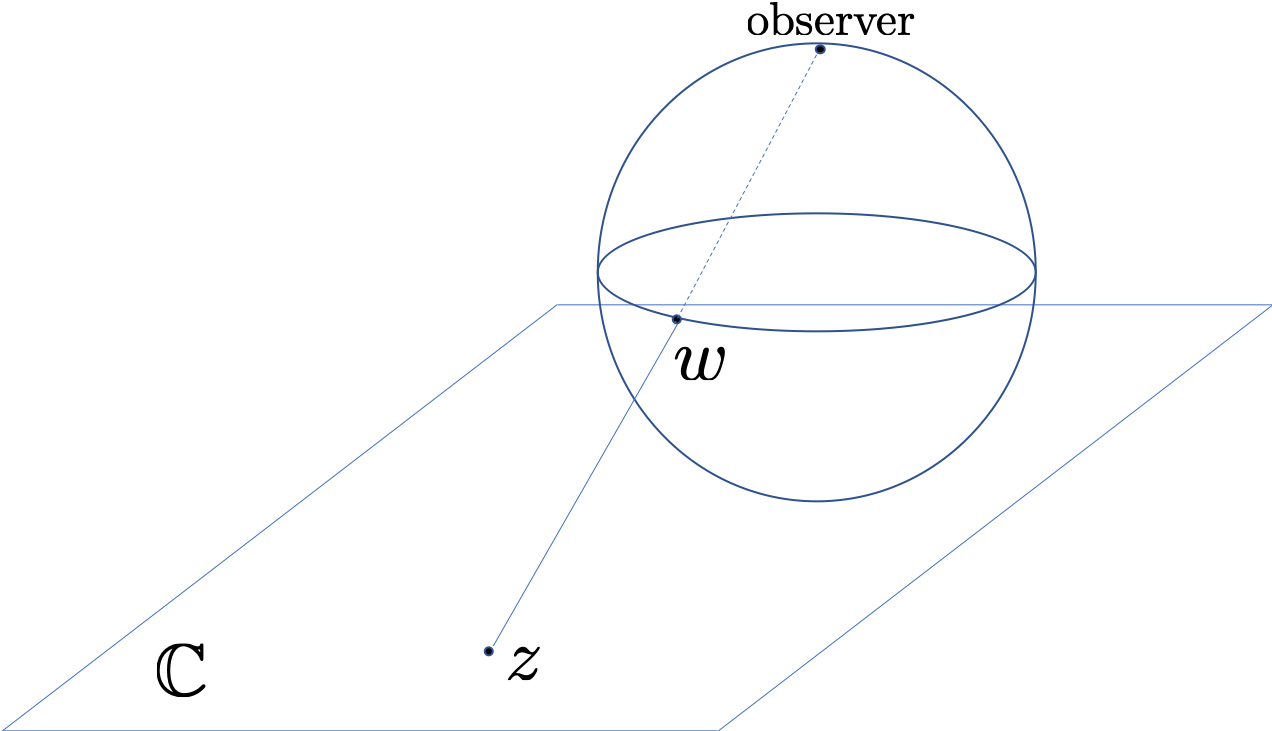
\includegraphics[width=3in]{images/riemann_sphere.png} 
\end{figure} 

\noindent Where the conformal group is

\begin{equation}
\text{Conf}(\mathbb{C} \cup \{ \infty \} ) = \Big{\{} f(z) = \frac{\alpha z + \beta}{\gamma z + \delta}; \, \alpha, \beta, \gamma, \delta \in \mathbb{C}, \alpha\delta - \beta \gamma \ne 0 \Big{\}}.
\end{equation}

\noindent This is also called the group of Moebius transformations, and is a slightly larger group of conformal transformations (symmetires), since we can map to and from infinity as a point. \\

\subsubsection*{Summary}

\noindent A conformal field theory is a local quantum field theory that is invariant under the conformal group, a set of transformations, a change in coordinates, that leave the metric invariant up to a scale factor. In different spacetime dimensions, the conformal group takes on significantly different forms. \\

\noindent The global conformal group in dimensions greater than two is comprised of translations, rotations, scaling, and special conformal transformations, as well as dimensions equal to two, as long as the space is compactified. If singularities are included, functions with poles are allowed, the symmetry gets larger.